%% Manuscript for the effect of designed conversational architecture on the perception of agents
%%
%% The first command in your LaTeX source must be the \documentclass command.
\documentclass[sigconf,screen,review, anonymous]{acmart}

\usepackage[linewidth=1pt]{mdframed}
\usepackage{lipsum}
\usepackage{multirow}
\usepackage{graphicx}
\usepackage{booktabs}
\usepackage{makecell} 

\newcommand{\cmt}[1]{}%{\ignorespaces}


%% NOTE that a single column version may be required for 
%% submission and peer review. This can be done by changing
%% the \doucmentclass[...]{acmart} in this template to 
%% \documentclass[manuscript,screen]{acmart}
%% 
%% To ensure 100% compatibility, please check the white list of
%% approved LaTeX packages to be used with the Master Article Template at
%% https://www.acm.org/publications/taps/whitelist-of-latex-packages 
%% before creating your document. The white list page provides 
%% information on how to submit additional LaTeX packages for 
%% review and adoption.
%% Fonts used in the template cannot be substituted; margin 
%% adjustments are not allowed.
%%
%%
%% \BibTeX command to typeset BibTeX logo in the docs
\AtBeginDocument{%
  \providecommand\BibTeX{{%
    \normalfont B\kern-0.5em{\scshape i\kern-0.25em b}\kern-0.8em\TeX}}}

%% Rights management information.  This information is sent to you
%% when you complete the rights form.  These commands have SAMPLE
%% values in them; it is your responsibility as an author to replace
%% the commands and values with those provided to you when you
%% complete the rights form.
\setcopyright{acmcopyright}
\copyrightyear{2023}
\acmYear{2023}
\acmDOI{XXXXXXX.XXXXXXX}

%% These commands are for a PROCEEDINGS abstract or paper.
\acmConference[Conference acronym 'XX]{Make sure to enter the correct
  conference title from your rights confirmation email}{June 03--05,
  2018}{Woodstock, NY}
%
%  Uncomment \acmBooktitle if th title of the proceedings is different
%  from ``Proceedings of ...''!
%
%\acmBooktitle{Woodstock '18: ACM Symposium on Neural Gaze Detection,
%  June 03--05, 2018, Woodstock, NY} 
\acmPrice{15.00}
\acmISBN{978-1-4503-XXXX-X/18/06}

%%
%% Submission ID.
%% Use this when submitting an article to a sponsored event. You'll
%% receive a unique submission ID from the organizers
%% of the event, and this ID should be used as the parameter to this command.
%%\acmSubmissionID{123-A56-BU3}

%%
%% end of the preamble, start of the body of the document source.
\begin{document}
%TC:ignore

%%
%% The "title" command has an optional parameter,
%% allowing the author to define a "short title" to be used in page headers.
% \title[short title]{How to Make Pinocchio a Real Boy? Designing conversational architecture elements to achieve desirable anthropomorphized perceptions}
\title[The Bot with the Eloquent Speech]{The Bot with the Eloquent Speech: Exploring the Relationship between Perceptions of Conversational Agents and Their Conversation Architecture}

%%
%% The "author" command and its associated commands are used to define
%% the authors and their affiliations.
%% Of note is the shared affiliation of the first two authors, and the
%% "authornote" and "authornotemark" commands
%% used to denote shared contribution to the research.
\author{Christina Wei}
\email{christina.wei@mail.utoronto.ca}
\affiliation{%
  \institution{University of Toronto}
  \city{Toronto}
  \country{Canada}
}

\author{Young-Ho Kim}
\email{ygho.kim@navercorp.com}
\affiliation{%
  \institution{Naver Corporation}
  \city{Seoul}
  \country{Korea}
}

\author{Anastasia Kuzminykh}
\email{anastasia.kuzminykh@utoronto.ca}
\affiliation{%
  \institution{University of Toronto}
  \city{Toronto}
  \country{Canada}
}

%%
%% By default, the full list of authors will be used in the page
%% headers. Often, this list is too long, and will overlap
%% other information printed in the page headers. This command allows
%% the author to define a more concise list
%% of authors' names for this purpose.
\renewcommand{\shortauthors}{Wei, Kim, and Kuzminykh}

%%
%% The abstract is a short summary of the work to be presented in the
%% article.
\begin{abstract}
Previous research has demonstrated a relationship between the structure of conversational agents' natural language interaction and how these agents are perceived by their users. However, the systematic connections between the perception of agents and elements of conversation architecture are not well understood. Furthermore, there is no clear definition of the aspects of perception that are affected and the elements of conversation architecture. In this paper, we present a synthesized framework demonstrating the connections between perceptions of agents and conversation architecture elements, using a taxonomy of eleven perceptions grouped into four categories, and ten elements grouped into three categories. We highlight the need for further research for the perception of agent's ability and perception of social connection with agent's, especially as it relates to the linguistic style of conversational agents.  Also, there is the need to be consistent in the assessment of agents' perceptions, and address ethical concerns in design.
\end{abstract}

%%
%% The code below is generated by the tool at http://dl.acm.org/ccs.cfm.
%% Please copy and paste the code instead of the example below.
%%
\begin{CCSXML}
<ccs2012>
 <concept>
  <concept_id>10010520.10010553.10010562</concept_id>
  <concept_desc>Computer systems organization~Embedded systems</concept_desc>
  <concept_significance>500</concept_significance>
 </concept>
 <concept>
  <concept_id>10010520.10010575.10010755</concept_id>
  <concept_desc>Computer systems organization~Redundancy</concept_desc>
  <concept_significance>300</concept_significance>
 </concept>
 <concept>
  <concept_id>10010520.10010553.10010554</concept_id>
  <concept_desc>Computer systems organization~Robotics</concept_desc>
  <concept_significance>100</concept_significance>
 </concept>
 <concept>
  <concept_id>10003033.10003083.10003095</concept_id>
  <concept_desc>Networks~Network reliability</concept_desc>
  <concept_significance>100</concept_significance>
 </concept>
</ccs2012>
\end{CCSXML}

\ccsdesc[500]{Computer systems organization~Embedded systems}
\ccsdesc[300]{Computer systems organization~Redundancy}
\ccsdesc{Computer systems organization~Robotics}
\ccsdesc[100]{Networks~Network reliability}

%%
%% Keywords. The author(s) should pick words that accurately describe
%% the work being presented. Separate the keywords with commas.
\keywords{conversational agents, user perception, conversational architecture, anthropomorphized perceptions, social cues}

%%\received{20 February 2007}
%%\received[revised]{12 March 2009}
%%\received[accepted]{5 June 2009}

%%
%% This command processes the author and affiliation and title
%% information and builds the first part of the formatted document.
\maketitle
%TC:endignore


%%%% TODO %%%%
% Add headmap of explored relationships - side by side with the connections - show numbers - DONE
% Put the heatmap of impact earlier in the paper - DONE
% Put the tables together - DONE
% show what is explored vs. the connections that had impacts. - DONE
% User perception of agent instead of anthropomorphized perceptions
% Refer to the explored connection in writing, and connections with impacts
% Update to use perception aspects and categories (instead of themes and organizing themes)
% Update introduction
% Include focus areas for future reasearch
% Reviewed recording up to 17:31
% Question about single column vs. double column format - ask Jaisie

\section{Introduction}

Conversational agents (CAs) are software-based systems, either voice of text-based, designed to interact with humans using natural language. Adoption for CAs such as Alexa (Amazon) or Siri (Apple) are rapidly growing in the market, with half of US internet users own one or more smart speaker devices \cite{2022comscore}. These conversational agents are designed to be ubiquitous, easily accessible through smartphones, tablets, laptops and smart devices. Because these agents leverage natural language for interaction, they solicit social responses from users, encouraging users to attribute lifelike qualities, a.k.a. anthropomorphized perceptions to CAs \cite{eyssel2012if}.

Anthropomorphism is defined as the attribution of traits that we typically associate with being distinctly human to nonhuman entities \cite{waytz2010sees}. For example, users tend to personify conversational agents like Amazon Alexa by using person pronouns instead of object pronouns in online reviews \cite{purington2017alexa}.  Research shows that anthropomorphic design is beneficial to establishing and maintaining trust between users and conversational agents \cite{seeger2021chatbots}. Also, speakers tend to align their lexical choices with conversational agents, similar to human-human conversations \cite{cowan2015does}. Anthropomorphism has been shown to ease user interactions, e.g. making agents more approachable, engaging, and trustworthy when they exhibit human characteristics \cite{qiu2009evaluating}. These processes are of particular interest for human-agent communication because they form the basis for user expectations and predispositions regarding agents' behavior, reliability of the information, etc. \cite{kuzminykh2020genie}.

One of the key factors for anthropomorphized perception is how conversational agents convey information through verbal or non-verbal cues. Studies have found that conversational agents are perceived as more socially present and emotionally intelligent if they use affect language such as sentiment-adaptive response based on user's utterances, resulting in higher user satisfaction \cite{diederich2019emulating}\cite{yang2017perceived}. Also, CAs that mimic user behaviour through lexical alignment reduce users' cognitive workload, resulting in higher engagement with the interaction \cite{spillner2021talk}. Non-linguistic cues such as expressive prosody contribute to higher perceived intimacy with the user, as well as higher perceived enjoyment and ease of use \cite{kim2020can}. While there is existing research on the impact of conversation architecture on anthropomorphized perceptions of agents, their findings are hard to generalize due to obstacles in consistency of taxonomy and measures.
%However, conversational architecture design may lead to negative consequences, such as an agent with an extroverted personality may be seen as less trustworthy, as users are irritated by the system's overly familiar attitude \cite{andrews2012system}.

 There have been recent efforts to systematically analyze UX measurements used to evaluate conversational agents. In Clark et al's review for the state of speech interfaces, the authors created a list the different concepts used to measure disembodied voice-based agents such as user attitudes and task performance \cite{clark2019state}. Rapp et al. \cite{rapp2021human} analyzed literature related specifically to text-based CAs, where the themes emerged from their analysis has aspects related to the anthropomorphized perceptions, like humanness and emotional experience. Most recently, Zheng et al's literature review on the UX research of CAs \cite{zheng2022ux} categorized the metrics based on the type of method used, including technical measures like system error rate and perception measures like perceived social presence. Specifically to measures related to anthropomorphized perceptions, there is a gap of research to systematically analyze the different aspects of these perceptions, as well as a consistent taxonomy to refer to them. Similarly for conversation architecture elements, there is existing research to systematically analyze them, like Feine et al \cite{feine2019taxonomy}'s overall framework provides consistent categories for social cues. However, it is unknown which conversation architecture elements have impacts on the perceptions of agents. Lastly, while there are various studies investigating the effect of  conversational architecture elements on the anthropomorphized perception of agents, we did not find any systematic review and analysis to generalize the findings into a usable framework.

We are addressing this research gap by analyzing how to design conversation architecture in order to orchestrate anthropomorphized perceptions of conversational agents. First, we want to understand (RQ1) what aspects of anthropomorphized perceptions are being explored that are affected by conversation architecture. Conversation architecture has various aspects that affect a CA's utterances such as the use of humour, emoticons, or lexical alignment. This leads to our second research question: (RQ2) what are the elements of conversation architecture that are relevant to anthropomorphized perceptions? Lastly, we want to understand the impact of conversation architecture on perceptions of agent, which leads to our third research question: (RQ3) what are the relationships between the specifics of conversation architecture elements and the anthropomorphized perceptions of CAs?

To answer these questions, we need to synthesize existing literature by performing a comprehensive review from 2010 to 2022 on the impact of conversation architecture elements on anthropomorphized perceptions of CAs (n=57). We collected perceptions that are affected by conversation architecture and grouped them into four categories and eleven themes (Table \ref{tab:perceptions}). Similarly, we analyzed the conversation architecture elements explored in literature and grouped them into three categories and ten themes (Table \ref{tab:cues}). Lastly, we coded the explored connections between conversation architecture and perceptions and demonstrated the impacted relationship into a generalized framework (Figure \ref{fig:heatmap-impact}). Through our analysis, we also found that there are inconsistencies on how anthropomorphized perceptions are measured across studies, as well as influencing factors other than conversation architecture that may be impacting the perceptions of agents.

This work contributes to the HCI community by presenting an in-depth analysis on the impact of conversation architecture on anthropomorphized perceptions. We created a taxonomy for perceptions and conversation architecture elements to provide consistent terms that can be used in future research. Also, our analysis extends existing reviews on UX research of CAs \cite{clark2019state}\cite{rapp2021human}\cite{zheng2022ux} by providing a generalized framework outlining the relationships between conversation architecture and anthropomorphized perceptions. This framework provides the foundational knowledge to design conversation agents to solicit specific social responses from users.

In the remainder of the paper, we first outline our literature review and data analysis process, as well as the characteristics of the papers in our reviewed corpus. Following that, we describe in detail the taxonomy of anthropomorphized perceptions, taxonomy of conversation architecture element, as well as the framework on the relationships between perceptions and conversation architecture. Finally, we discuss the research challenges and opportunities as well as ethical considerations for designing conversational architecture to orchestrate anthropomorphized perceptions of conversational agents.


%\section{Literature Review}

%\cite{finch2020towards} Towards unified dialogue system evaluation: A comprehensive analysis of current evaluation protocols


\section{Methods}

This section describes the research methodologies for the search procedure, selection criteria and data analysis process.

\subsection{Data Collection}

Following PRISMA guidelines \cite{prisma}, we reviewed and selected literature relevant to the relationships between the specifics of conversation architecture elements and anthropomorphized perceptions of CAs. Searches were carried out in the ACM Digital Library between January 1 and January 15, 2023. During initial analysis, it didn't seem like there were common terms used to refer to either conversation architecture elements, or anthropomorphized perceptions. As such, search terms were kept general to literature related to conversational agents. Based on search terms used in previously published literature reviews \cite{clark2019state}\cite{rapp2021human} , the following keywords have been identified to search for publications related to conversational user interfaces:
\newline

\textit{"conversational agent" OR "natural language interface" OR "IPA" OR "intelligent personal assistant" OR "chatbot" OR "speech interface" OR "voice assistant" OR "intelligent agent" OR "human-chatbot communication" OR "virtual agent" OR "dialog* system" OR "voice user interface" OR "human computer dialog*"}
\newline

The initial query retrieved 2901 unique publications. The following selection criteria are applied to identify literature related to the effect of conversational architecture on perception of agents:
\begin{itemize}
  \item Peer-reviewed publications written in English
  \item Voice-based or text-based conversational agents
  \item Experiment study on the impact of conversation architecture elements on the anthropomorphized perceptions of agents
  \item Impact of conversation architecture elements can be separated from other effects (e.g. embodiment)

\end{itemize}

We screened the titles and abstracts of the papers based on the selection criteria below which resulted in 221 papers. Reviewing the full articles of these publication resulted in 49 papers for analysis. An additional search for related literature was also performed to find new publications, adding 8 more papers to the corpus. We identified 57 relevant articles that met our selection criteria (see Figure \ref{fig:prisma}).

\begin{figure}[h]
  \centering
  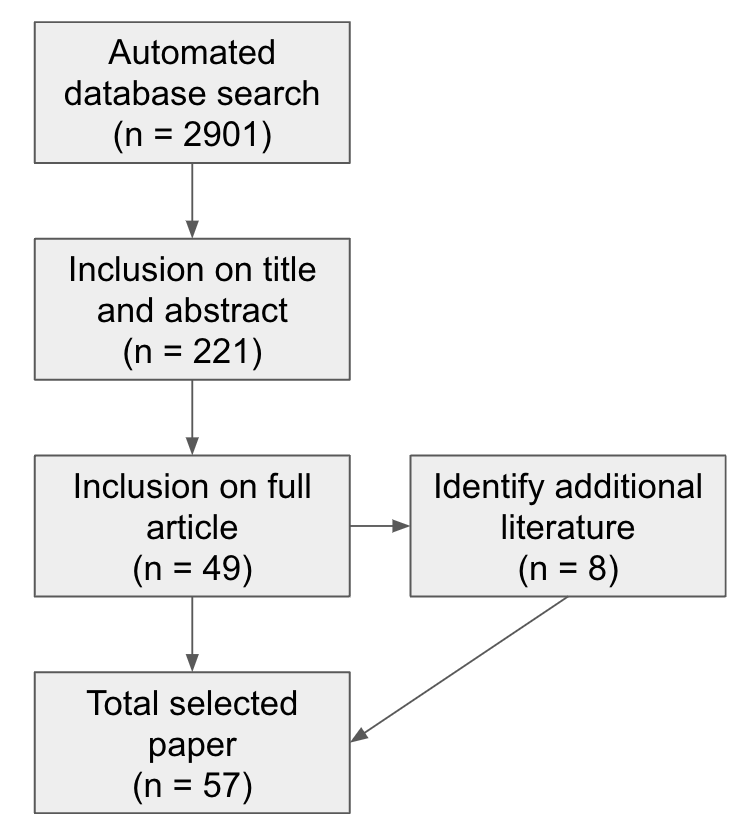
\includegraphics[width=1\columnwidth]{fig-prisma.png}
  \caption{Literature search using PRISMA guidelines}
  \label{fig:prisma}
\end{figure}

\subsubsection*{Literature Corpus Characteristics}

The papers reviewed (n=57) were published between May 2011 and November 2022. More than 75\% of the papers were published in or after 2019, with a slight trend upwards over the years (see Figure \ref{fig:paper}). The vast majority of the papers in our corpus were published in conference proceedings (n=50), with the remainder papers published in journals. Out of the papers published in conferences, the top conferences were The ACM Conference on Human Factors in Computing Systems\footnote{https://dl.acm.org/conference/chi} (n=16), Conversational User Interfaces\footnote{https://dl.acm.org/conference/cui} (n=7), Human-Agent Interaction\footnote{https://dl.acm.org/conference/hai} (n=4), and Intelligent Virtual Agents\footnote{https://dl.acm.org/conference/iva} (n=4). 
%Out of the papers published in journals, some venues include the International Journal of Human-Computer Interaction\footnote{https://www.tandfonline.com/journals/hihc20} (n=2) and Interacting with Computers\footnote{https://academic.oup.com/iwc} (n=1).

On the modality characteristics of the conversational agents in the corpus, there is a roughly even split between the modalities, with slightly more papers (n=30) studying voice-based CAs, and the rest (n=27) studying text-based CAs.

\begin{figure}[h]
  \centering
  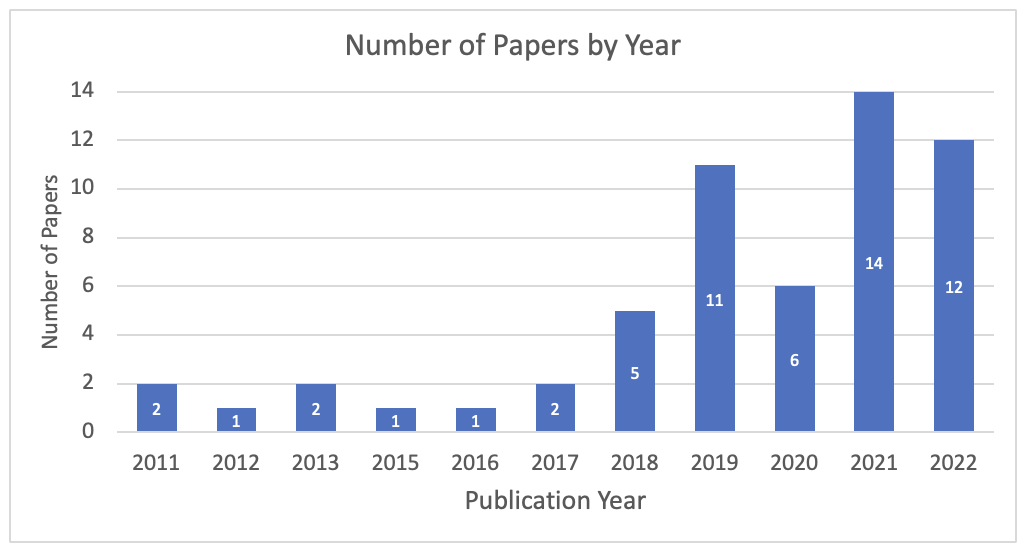
\includegraphics[width=\columnwidth]{fig-paper.png}
  \caption{Number of papers by year}
  \label{fig:paper}
\end{figure}

\subsection{Data Analysis}

\subsubsection*{Anthropomorphized Perceptions} To study RQ1, the exact quotes of anthropomorphized perception measurements were extracted from each paper. Inductive thematic analysis was used to group these verbatim quotes into codes based on their meanings. For example, the code likeability of the agent contains the questionnaire item "this voice agent was likeable" used by \cite{cuadra2021my}\cmt{[67]}, Godspeed questionnaire \cite{bartneck2009measurement}\cmt{godspeed}'s set of questions on likeability used by \cite{linnemann2018can}\cmt{[15]}, and Subjective Assessment of Speech System Interface (SASSI) questionnaire \cite{hone2000towards}\cmt{sassi}'s set of questions on likeability used by  \cite{chan2021kinvoices}\cmt{[74]}\cite{choi2020nobody}\cmt{[54]}. This step resulted in 83 unique codes. The codes are then organized based similarity of the meanings, resulting in 11 basic themes. For example, the basic theme of \textit{personality traits} of the agent contains measurements such as likeability, friendliness, and warmth. Lastly, the 11 basic themes are categorized into 4 organizing themes: \textit{perception of interaction with agent, perception of agent's ability, perception of social connection with agent, and perception of agent's humanness} (Table \ref{tab:perceptions}).

\subsubsection*{Conversation Architecture Elements}
The study RQ2, the conversation architecture elements used in the study were extracted from each paper. Some of the papers were applying multiple elements to the CA design, such as the the anthropomorphic design used in this study \cite{seeger2021chatbots}\cmt{[35]}. In the case where multiple elements were used, the codes broke down the conversation architecture into its core components. For example, the anthropomorphic design used in Seeger et al's study \cite{seeger2021chatbots}\cmt{[35]} was broken down to the elements of emotional expressions, is-typing indicator, emoticons, and response delay to capture as codes. 58 unique codes were created as part of this process, capturing elements like sentiment-adaptive responses \cite{diederich2019emulating}\cmt{[25]}, lexical alignment \cite{spillner2021talk}\cmt{[18]}, and typos \cite{westerman2019believe}\cmt{[9]}. Codes were then organized based on similarity of the elements. For example, the basic theme of \textit{disfluency} contains elements of fillers \cite{jeong2019exploring}\cmt{[10]}\cite{wester2015artificial}\cmt{[14]}, interjections \cite{ceha2022expressive}\cmt{[77]}\cite{hu2021enhancing}\cmt{[56]}, and repetitions \cite{yang2021effect}\cmt{[72]}. Lastly, these basic themes are then categorized into organizing themes adapted from the social cues taxonomy structure by Feine et al \cite{feine2019taxonomy}. Based on this paper, the Verbal-Content category is mapped to our organizing theme of \textit{linguistic content}, and the Verbal-Style category is mapped to our organizing theme of \textit{linguistic style}.
Given our analysis focuses on the text and voice aspects of a conversational agent and does not analyze the embodiment aspects of design, the visual category is not applicable for our analysis. Also, we collapsed the auditory and invisible categories into the organizing theme of \textit{non-linguistic format} (Table \ref{tab:cues}).

\subsubsection*{Relationship Between Anthropomorphized Perceptions and Conversation Architecture Elements}
For RQ3, we extracted the relationships between perceptions and architecture elements from each paper based on the codes developed for anthropomorphized perceptions and conversation architecture elements above, noting whether the architecture element had an impact of on the perceptions. Out of the 57 papers, 264 connections between anthropomorphized perceptions and conversation architecture elements were found. To analyze specifically the relationships between the specifics of conversation architecture that affect the anthropomorphized perceptions of CAs, 69 connections that did not result in significant relationships were discarded, resulting in 195 relationships for analysis. For example, the specific connection between style matching and user satisfaction was discarded because Hoegen et al. \cite{hoegen2019end}\cmt{[31]} did not find a significant difference between the style matching agent and the non-style matching agent for overall interaction satisfaction. Out of the 195 relationships, 185 were relationships between individual architecture elements and perceptions. These single architecture element to perception relationships are visualized as a heatmap based on literature coverage within the literature review corpus, as seen in Figure \ref{fig:heatmap-impact}. Perceptions impacted by the composite of multiple architecture elements in an agent will be discussed in more details in the Composite Architecture Elements section.

\section{Findings}

\begin{figure*}[]
  \centering
  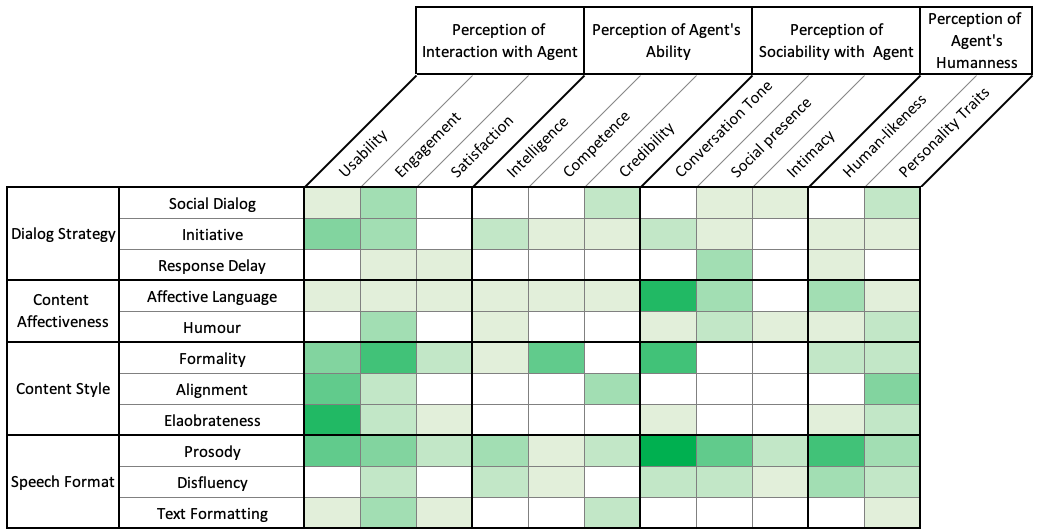
\includegraphics[width=\textwidth]{fig-heatmap-impact.png}
  \caption{Heatmap of literature for perception of conversational agents for each type of conversational architecture element}
  \label{fig:heatmap-impact}
\end{figure*}

\subsection{Anthropomorphized Perceptions}

As shown in Table \ref{tab:perceptions}, there are four organizing themes defined for the anthropomorphized perceptions of conversational agents covering 11 basic themes of perception. The details of each theme are discussed below.

\textbf{Perception of interaction with agent} evaluates the overall interaction quality users had with the conversational agent. The three basic themes for this perceptions are usability, engagement and satisfaction. \textit{Usability} measures the utilitarian aspects of the interaction, whether it was accurate, easy to use, efficient or helpful. Some commonly used methods to measure usability include the response accuracy portion of the SASSI questionnaire \cite{hone2000towards}\cmt{sassi}, or the NASA Task Load Index (NASA-TLX) \cite{hart1988development}\cmt{nasa} to measure cognitive workload. Questions such as "the system is easy to use" or "it is easy to understand the agent" are also measures of usability. \textit{Engagement} on the other hand measures users' emotional reactions, whether they have enjoyed the conversation with CA, or annoyed or frustrated with the interaction. Some commonly used methods to measure engagement include  the annoyance portion of the SASSI questionnaire \cite{hone2000towards}\cmt{sassi}, and the Use Engagement Scale (UES) \cite{o2018practical}\cmt{ues}. Questions such as "I enjoyed using the system" or "I felt frustrated with the agent" are also measures of engagement. Lastly, \textit{Satisfaction} measures users' overall satisfaction interacting with the agent. Questions such as "the overall assessment of conversing with the CA was satisfactory" are used to measure this perception.

\textbf{Perception of agent's ability} evaluates the perceived capabilities of the agent. While there are some elements of system performance in this measure, the main aspect we are interested in is the perception differences for agents with identify system capabilities but with different architecture elements. Specifically, \textit{intelligence} measures the agent's expertise and knowledge, and it is commonly administered through the Godspeed questionnaire \cite{bartneck2009measurement}\cmt{godspeed} on the set of questions related to perceived intelligence. Also survey questions such as asking users about the agent's intelligence and domain knowledge are used to measure perceived intelligence. \textit{Competence} takes intelligence one step further by evaluating the agent's ability to put its intelligence into practice. To measure a CA's competence, there are usually surveys or qualitative feedback that the agent is capable and competent, and that the users have confidence in the agent's ability to get the job done. Lastly, \textit{trust} evaluates agent's truthfulness, credibility and benevolence. Some commonly used methods to evaluate trust include the Trust Propensity Scale \cite{mayer1999effect} and the Individualized Trust Scale (ITS) \cite{wheeless1977measurement}. Questions such as "is the agent honest" and "can I trust the agent with sensitive information" are also measures of trust.

\textbf{Perception of the social connection with agent} evaluates the emotional connections that users have with agents. The three basic themes of conversation tone, social presence and intimacy are included in this category. \textit{Conversation tone} measure the affective impression of the agent's tone, such as empathy, expressiveness, or passionate. Also, it measures whether the tone used by the agent is persuasive or appropriate for the conversation. \textit{Social presence} measures the sense of connectness and psychological distance users has with an agent. Some aspects in this measure include a sense of familiarity or similarity with the agent, whether users feel the agent behaves like them or have similar attitudes to them. The measure of \textit{Intimacy} extends social presence into the realm of the quality of relationships with an agent. Some commonly used measures include the set of social attraction questions from the interpersonal attraction questionnaire \cite{mccroskey1975development} and the quality of relationship inventory (QRI) \cite{pierce1997assessing}. These questionnaires include questions like "I think the agent could be a friend of mine", or "I feel we could establish a personal relationship with each other".

\textbf{Perception of agent's humanness} evaluates human-likeness and the anthropomorphized personality traits that users assign to agents. \textit{Human-likeness} measures whether the agent presented itself as natural and human-like, or artificial and machine-like. The Godspeed questionnaire \cite{bartneck2009measurement}\cmt{godspeed} set of questions related to anthropomorphism and the Ascent of Man scale \cite{kteily2015ascent} are commonly used methods to assess human-likeness. Survey questions with semantic scales such as "human-like / machine-like" and "artificial / natural" are also used for this perception. \textit{Personality traits} captures the human characteristics that are attributes to the agent, such as warm, friendly, likeable, and polite. This is commonly captured in the qualitative feedback from users, commenting on whether the agent is extroverted or introverted, or the human characteristics they perceive the agent such as funny or witty. Some studies used the measure of the Big-5 personality traits \cite{gosling2003very} to map an agent's disposition on various personality dimensions.

Overall there is good coverage of perception measures based on the list of papers reviewed in our corpus. The most commonly measured perceptions are related to the interaction with agent, followed by the perception of agent's humanness. There are two basic themes that are the least measured compared to the others: competence under the perception of agent's ability, and intimacy under the perception of social connection with agent. This may be due to the controlled lab settings for the experiments, where participants are given the scenarios for interaction. This environment is not conducive to forming relationships with a conversational partner, as noted by Linnerman et al. in their discussions \cite{linnemann2018can}\cmt{[15]}. Also, the same factor could impact the assessment of agent's abilities, as the users may not feel like they have the expertise to assess an agent's competence. These factors could contribute to the reasons why competency and intimacy are not as frequently measured in experimental studies.

% Add citations

\begin{table*}[ht]
\renewcommand*{\arraystretch}{1.4}
\resizebox{\textwidth}{!}{%
\begin{tabular}{@{}p{0.17\textwidth} | p{0.12\textwidth} | p{0.20\textwidth} | >{\centering}p{0.09\textwidth} | p{0.42\textwidth} @{}}
%!{\vrule width 1.2pt} 
\Xhline{1.2pt}
\multicolumn{2}{l|}{\textbf{Perception Aspects}} & \textbf{Examples} & \textbf{No. Papers} & \textbf{Papers} 
\\ \Xhline{1.2pt}
\multirow{3}{*}{\parbox{0.16\textwidth}{Perception of Interaction with Agent}}
    & Usability & accuracy, ease of use, efficiency, helpfulness & 23 
    & \cite{ashktorab2019resilient}\cmt{[88]}\cite{ceha2022expressive}\cmt{[77]}\cite{chan2021kinvoices}\cmt{[74]}\cite{choi2020nobody}\cmt{[54]}\cite{cuadra2021my}\cmt{[67]}\cite{dubiel2020persuasive}\cmt{[60]}\cite{elsholz2019exploring}\cmt{[61]}\cite{haas2022keep}\cmt{[78]}\cite{habler2019effects}\cmt{[63]}\cite{healey2013relating}\cmt{[39]}\cite{hu2022polite}\cmt{[76]}\cite{huiyang2022improving}\cmt{[17]}\cite{jestin2022effects}\cmt{[81]}\cite{kim2019comparing}\cmt{[89]}\cite{kim2020can}\cmt{[24]}
    \cite{kraus2020effects}\cmt{[64]}\cite{linnemann2018can}\cmt{[15]}\cite{ma2022ask}\cmt{[29]}\cite{miehle2018exploring}\cmt{[51]}\cite{misu2011toward}\cmt{[83]}\cite{roy2021users}\cmt{[71]}\cite{spillner2021talk}\cmt{[18]}\cite{wilhelm2022keep}\cmt{[28]}
\\ \cline{2-5}
    & Engagement & enjoyment, annoyance, desirable, intention to use  & 28
    & \cite{andrews2012system}\cmt{[38]}\cite{ceha2022expressive}\cmt{[77]}\cite{ceha2021can}\cmt{[57]}\cite{chan2021kinvoices}\cmt{[74]}\cite{cox2022does}\cmt{[27]}\cite{cuadra2021my}\cmt{[67]}\cite{elsholz2019exploring}\cmt{[61]}\cite{fadhil2018effect}\cmt{[52]}\cite{gnewuch2022opposing}\cmt{[20]}\cite{go2021conversational}\cmt{[80]}\cite{healey2013relating}\cmt{[39]}\cite{huiyang2022improving}\cmt{[17]}\cite{jestin2022effects}\cmt{[81]}\cite{kim2020can}\cmt{[24]}\cite{kim2019comparing}\cmt{[89]}
    \cite{lee2020hear}\cmt{[23]}\cite{linnemann2018can}\cmt{[15]}\cite{ma2022ask}\cmt{[29]}\cite{miehle2018exploring}\cmt{[51]}\cite{miyamoto2017improving}\cmt{[46]}\cite{moilanen2022measuring}\cmt{[82]}\cite{roy2021users}\cmt{[71]}\cite{spillner2021talk}\cmt{[18]}\cite{volkel2021examining}\cmt{[69]}\cite{volkel2022user}\cmt{[75]}\cite{xiao2021let}\cmt{[73]}\cite{yang2021effect}\cmt{[72]}\cite{zhu2022effects}\cmt{[26]}    
\\ \cline{2-5}
    & Satisfaction & service satisfaction, quality of interaction & 12
    & \cite{ceha2022expressive}\cmt{[77]}\cite{choi2020nobody}\cmt{[54]}\cite{diederich2019emulating}\cmt{[25]}\cite{elsholz2019exploring}\cmt{[61]}\cite{habler2019effects}\cmt{[63]}\cite{gnewuch2018faster}\cmt{[19]}\cite{hoegen2019end}\cmt{[31]}\cite{hu2022polite}\cmt{[76]}\cite{ma2022ask}\cmt{[29]}\cite{roy2021users}\cmt{[71]}\cite{wilhelm2022keep}\cmt{[28]}\cite{yang2017perceived}\cmt{[44]}
\\ \Xhline{1.2pt} 
\multirow{3}{*}{\parbox{0.16\textwidth}{Perception of Agent's Ability}}
    & Intelligence & knowledgeable, intelligent, expertise & 11
    & \cite{ashktorab2019resilient}\cmt{[88]}\cite{ceha2021can}\cmt{[57]}\cite{chan2021kinvoices}\cmt{[74]}\cite{cuadra2021my}\cmt{[67]}\cite{dubiel2020persuasive}\cmt{[60]}\cite{feijoo2021effects}\cmt{[70]}\cite{hu2021enhancing}\cmt{[56]}\cite{jeong2019exploring}\cmt{[10]}\cite{spillner2021talk}\cmt{[18]}\cite{volkel2022user}\cmt{[75]}\cite{yang2017perceived}\cmt{[44]} 
\\ \cline{2-5}
    & Competence & competent, capable & 4 
    & \cite{cox2022does}\cmt{[27]}\cite{kraus2020effects}\cmt{[64]}\cite{lee2019s}\cmt{[55]}\cite{westerman2019believe}\cmt{[9]}
\\ \cline{2-5}
    & Trust & credibility, trustworthy, truthfulness, confidence & 15
    & \cite{andrews2012system}\cmt{[38]}\cite{chan2021kinvoices}\cmt{[74]}\cite{dubiel2020persuasive}\cmt{[60]}\cite{fadhil2018effect}\cmt{[52]}\cite{healey2013relating}\cmt{[39]}\cite{hoegen2019end}\cmt{[31]}\cite{huiyang2022improving}\cmt{[17]}\cite{jestin2022effects}\cmt{[81]}\cite{kraus2020effects}\cmt{[64]}\cite{lee2020hear}\cmt{[23]}\cite{linnemann2018can}\cmt{[15]}\cite{ma2022ask}\cmt{[29]}\cite{seeger2021chatbots}\cmt{[35]}\cite{tolmeijer2021female}\cmt{[62]}\cite{wilhelm2022keep}\cmt{[28]}    
\\ \Xhline{1.2pt} 
\multirow{3}{*}{\parbox{0.16\textwidth}{Perception of Social Connection with Agent}}
    & Conversation Tone & appropriate, expressive, empathetic, persuasive & 13 
    & \cite{chan2021kinvoices}\cmt{[74]}\cite{cox2022does}\cmt{[27]}\cite{cuadra2021my}\cmt{[67]}\cite{daher2020empathic}\cmt{[58]}\cite{diederich2019emulating}\cmt{[25]}\cite{dubiel2020persuasive}\cmt{[60]}\cite{hu2021enhancing}\cmt{[56]}\cite{jestin2022effects}\cmt{[81]}\cite{misu2011toward}\cmt{[83]}\cite{tolmeijer2021female}\cmt{[62]}\cite{yang2021effect}\cmt{[72]}\cite{yang2017perceived}\cmt{[44]}\cite{zhu2022effects}\cmt{[26]}
\\ \cline{2-5}
    & Social Presence & connectedness, familiarity, psychological distance & 18
    & \cite{ceha2022expressive}\cmt{[77]}\cite{ceha2021can}\cmt{[57]}\cite{chan2021kinvoices}\cmt{[74]}\cite{choi2020nobody}\cmt{[54]}\cite{cuadra2021my}\cmt{[67]}\cite{diederich2019emulating}\cmt{[25]}\cite{gnewuch2018faster}\cmt{[19]}\cite{gnewuch2018chatbot}\cmt{[21]}\cite{gnewuch2022opposing}\cmt{[20]}\cite{go2021conversational}\cmt{[80]}\cite{khooshabeh2011does}\cmt{[37]}\cite{kim2020can}\cmt{[24]}\cite{lee2019s}\cmt{[55]}\cite{lubis2019positive}\cmt{[43]}\cite{lubold2016effects}\cmt{[86]}
    \cite{ma2022ask}\cmt{[29]}\cite{niewiadomski2013laugh}\cmt{[85]}\cite{westerman2019believe}\cmt{[9]}    
\\ \cline{2-5}
    & Intimacy & intimate, rapport, quality of relationship & 7 
    & \cite{choi2020nobody}\cmt{[54]}\cite{khooshabeh2011does}\cmt{[37]}\cite{kim2020can}\cmt{[24]}\cite{lee2020hear}\cmt{[23]}\cite{linnemann2018can}\cmt{[15]}\cite{lubold2016effects}\cmt{[86]}\cite{westerman2019believe}\cmt{[9]}
\\ \Xhline{1.2pt}
\multirow{2}{*}{\parbox{0.16\textwidth}{Perception of Agent's Humanness}}
    & Human-likeness & human-like, natural, artificial, machine-like & 20
    & \cite{ashktorab2019resilient}\cmt{[88]}\cite{ceha2021can}\cmt{[57]}\cite{chan2021kinvoices}\cmt{[74]}\cite{choi2020nobody}\cmt{[54]}\cite{cox2022does}\cmt{[27]}\cite{diederich2019emulating}\cmt{[25]}\cite{gnewuch2018faster}\cmt{[19]}\cite{haas2022keep}\cmt{[78]}\cite{hu2022polite}\cmt{[76]}\cite{jeong2019exploring}\cmt{[10]}\cite{jestin2022effects}\cmt{[81]}\cite{lubis2019positive}\cmt{[43]}\cite{ma2022ask}\cmt{[29]}\cite{misu2011toward}\cmt{[83]}\cite{niewiadomski2013laugh}\cmt{[85]}
    \cite{ouchi2019should}\cmt{[59]}\cite{seeger2021chatbots}\cmt{[35]}\cite{wester2015artificial}\cmt{[14]}\cite{westerman2019believe}\cmt{[9]}\cite{zhu2022effects}\cmt{[26]}    
\\ \cline{2-5}
    & Personality Traits & friendly, kind, warm, creepy, likeable, polite & 27
    & \cite{andrews2012system}\cmt{[38]}\cite{ashktorab2019resilient}\cmt{[88]}\cite{ceha2022expressive}\cmt{[77]}\cite{ceha2021can}\cmt{[57]}\cite{chan2021kinvoices}\cmt{[74]}\cite{cox2022does}\cmt{[27]}\cite{cuadra2021my}\cmt{[67]}\cite{haas2022keep}\cmt{[78]}\cite{habler2019effects}\cmt{[63]}\cite{healey2013relating}\cmt{[39]}\cite{hu2022polite}\cmt{[76]}\cite{huiyang2022improving}\cmt{[17]}\cite{jeong2019exploring}\cmt{[10]}\cite{jestin2022effects}\cmt{[81]}\cite{khooshabeh2011does}\cmt{[37]}
    \cite{kim2019comparing}\cmt{[89]}\cite{lee2019s}\cmt{[55]}\cite{lee2020hear}\cmt{[23]}\cite{linnemann2018can}\cmt{[15]}\cite{miehle2018exploring}\cmt{[51]}\cite{moilanen2022measuring}\cmt{[82]}\cite{ouchi2019should}\cmt{[59]}\cite{tolmeijer2021female}\cmt{[62]}\cite{volkel2021manipulating}\cmt{[68]}\cite{volkel2022user}\cmt{[75]}\cite{wester2015artificial}\cmt{[14]}\cite{zhu2022effects}\cmt{[26]} 
\\ \Xhline{1.2pt}
\end{tabular}%
}
\caption{Perception measures}
\label{tab:perceptions}
\end{table*}

\subsection{Conversation Architecture Elements}

As shown in Table \ref{tab:cues}, there are three categories defined for the conversation architecture elements covering 10 different themes. The details of each category and theme are discussed below.

The category of \textbf{linguistic content} maps to the content category under verbal cues in Feine et al's taxonomy, which refers to elements expressed with written or spoken words that are related to the strict and literal meaning of a message (i.e. what is said) \cite{feine2019taxonomy}. The theme of \textit{affective language} captures the injection of emotional words or phrases into the agent's utterance, such as affective expressions \cite{seeger2021chatbots}\cmt{[35]}\cite{yang2017perceived}\cmt{[44]}\cite{zhu2022effects}\cmt{[26]}, sentiment-adaptive responses \cite{diederich2019emulating}\cmt{[25]}, and encouraging words \cite{healey2013relating}\cmt{[39]}. \textit{Social talk} captures non-task related conversations with the user to build social connection, such as self-disclosure \cite{lee2020hear}\cmt{[23]} and social dialogue \cite{volkel2021manipulating}\cmt{[68]}\cite{lubold2016effects}\cmt{[86]}. The theme of \textit{humour} is similar to social talk but specific to CA's attempt to include jokes in its utterances. The separation of social talk and humor is based on findings from previous research, where user's attitude towards humour is different between human-human conversations vs. human-agent conversations \cite{clark2019makes}. We would like to capture the relationship between humour and agent perceptions differently from social talk. Lastly, the theme of \textit{agent-initiated content} captures utterances that are driven by the agent without direct prompts from the user. This elements in this theme include conversation repairs \cite{cuadra2021my}\cmt{[67]}\cite{ashktorab2019resilient}\cmt{[88]} and proactive content like eliciting feedback \cite{xiao2021let}\cmt{[73]}.

The category of \textbf{linguistic style} maps to the style category under verbal cues in Feine et al's taxonomy, which refers to elements expressed with written or spoken words that are related to the meaningful deployment of language variation in a message (i.e. how something is said) \cite{feine2019taxonomy}. The theme of \textit{formality} describes the language style used by the conversational agent, whether it is formal vs. casual, such as using honorific expressions to address users \cite{ouchi2019should}\cmt{[59]}. \textit{Alignment} captures the degree that the agent aligns its utterances to the users, such as lexical alignment on the content and structural of the sentences \cite{huiyang2022improving}\cmt{[17]}\cite{linnemann2018can}\cmt{[15]}, as well as agreement with the user \cite{volkel2021examining}\cmt{[69]}. \textit{Elaborateness} captures the sentence complexity and length of the utterances. For example, Roy et al. explored the differences in perception for variations in elaborateness such as "Cloudly, possibility of snow, high: 4, low: -10" vs "Today will be cloudy, with a high of 4 and a low of -10. Snow is predicted" \cite{roy2021users}\cmt{[71]}. Lastly, the category of \textit{disfluency} captures the style of using non-lexical utterances like filler words ("um, uh") \cite{hu2021enhancing}\cmt{[56]}\cite{jeong2019exploring}\cmt{[10]}, or repetition of words within a sentence \cite{yang2021effect}\cmt{[72]}. 

Lastly, the category of \textbf{non-linguistic format} maps loosely to the elements in auditory and invisible categories in Feine et al's taxonomy \cite{feine2019taxonomy}. These are auditory or textual variations in the presentation of the agent's utterances. In the theme of \textit{prosodic cue}, it captures vocal qualities like gender of voice \cite{habler2019effects}\cmt{[63]}\cite{jestin2022effects}\cmt{[81]}, and speech rate \cite{choi2020nobody}\cmt{[54]}. \textit{Text variations} include different formats that text-based agents use to present information to users, like emoticons \cite{kim2019comparing}\cmt{[89]}\cite{wilhelm2022keep}\cmt{[28]}, typos \cite{westerman2019believe}\cmt{[9]}, and response delays \cite{gnewuch2022opposing}\cmt{[20]}\cite{seeger2021chatbots}\cmt{[35]}.

Overall the spread of conversation architecture elements relevant to anthropomorphized perceptions are evenly distributed across linguistic content, linguistic style, and non-linguistic format.  Looking at the different themes, there is good coverage of studies on the impact of affective language and prosodic cues on anthropomorphized perceptions. However, it seemed like there is a lack of studies exploring the effect of agent-initiative content on the perception of agents. There are various existing literature on this theme such as conversation repairs \cite{komatani2010online}\cite{reinkemeier2022repair} and agent proactively sharing content with users \cite{dubiel2019inquisitive}\cite{zargham2022understanding}, but they were not included in this systematic literature review because they did not have measures of anthropomorphized perceptions of the CA. This may be because conversations with CAs have historically being driven by the user, with some recent effort to understand the opportunities to be more proactive \cite{cowan2023introduction}, as existing research are focused on the functional aspects of designing an agent instead of exploring into the anthropomorphized perceptions.


\begin{table*}[h]
\resizebox{\textwidth}{!}{
\renewcommand*{\arraystretch}{1.4}
\begin{tabular}{@{}p{0.17\textwidth} | p{0.14\textwidth} | p{0.25\textwidth} | >{\centering}p{0.09\textwidth} | p{0.34\textwidth} @{}}
\Xhline{1.2pt}
\textbf{Element Category} & \textbf{Element} & \textbf{Examples} & \textbf{No. Papers} & \textbf{Papers}
\\ \Xhline{1.2pt}
\multirow{4}{*}{Linguistic Content}    & Affective Language & emotional expressions, sentiment-adaptive responses & 11
& \cite{daher2020empathic}\cmt{[58]}\cite{diederich2019emulating}\cmt{[25]}\cite{healey2013relating}\cmt{[39]}\cite{hu2022polite}\cmt{[76]}\cite{lee2019s}\cmt{[55]}\cite{lubis2019positive}\cmt{[43]}\cite{moilanen2022measuring}\cmt{[82]}\cite{seeger2021chatbots}\cmt{[35]}\cite{volkel2022user}\cmt{[75]}\cite{yang2017perceived}\cmt{[44]}\cite{zhu2022effects}\cmt{[26]}
\\ \cline{2-5}
& Social Talk & self-disclosure, social dialogue & 7
& \cite{andrews2012system}\cmt{[38]}\cite{lee2020hear}\cmt{[23]}\cite{lubold2016effects}\cmt{[86]}\cite{moilanen2022measuring}\cmt{[82]}\cite{roy2021users}\cmt{[71]}\cite{volkel2021manipulating}\cmt{[68]}\cite{volkel2022user}\cmt{[75]}
\\ \cline{2-5}
& Humour & humorous content, jokes & 5
& \cite{ceha2021can}\cmt{[57]}\cite{go2021conversational}\cmt{[80]}\cite{khooshabeh2011does}\cmt{[37]}\cite{miyamoto2017improving}\cmt{[46]}\cite{volkel2021manipulating}\cmt{[68]}
\\ \cline{2-5}
& Agent-Initiated Content & proactive dialogue, conversation repair & 4
& \cite{ashktorab2019resilient}\cmt{[88]}\cite{cuadra2021my}\cmt{[67]}\cite{kraus2020effects}\cmt{[64]}\cite{xiao2021let}\cmt{[73]}
\\ \Xhline{1.2pt}
\multirow{4}{*}{Linguistic Style} & Formality & formal vs. casual, honorific expressions & 9
& \cite{cox2022does}\cmt{[27]}\cite{elsholz2019exploring}\cmt{[61]}\cite{habler2019effects}\cmt{[63]}\cite{jestin2022effects}\cmt{[81]}\cite{kim2019comparing}\cmt{[89]}\cite{ma2022ask}\cmt{[29]}\cite{moilanen2022measuring}\cmt{[82]}\cite{ouchi2019should}\cmt{[59]}\cite{volkel2022user}\cmt{[75]}
\\ \cline{2-5}
& Alignment & content matching, lexical alignment, agreeableness & 7
& \cite{healey2013relating}\cmt{[39]}\cite{hoegen2019end}\cmt{[31]}\cite{huiyang2022improving}\cmt{[17]}\cite{linnemann2018can}\cmt{[15]}\cite{spillner2021talk}\cmt{[18]}\cite{volkel2021examining}\cmt{[69]}\cite{volkel2021manipulating}\cmt{[68]}
\\ \cline{2-5}
& Elaborateness & elaborate, concise, sentence structure & 6
& \cite{haas2022keep}\cmt{[78]}\cite{miehle2018exploring}\cmt{[51]}\cite{moilanen2022measuring}\cmt{[82]}\cite{roy2021users}\cmt{[71]}\cite{volkel2021manipulating}\cmt{[68]}\cite{volkel2022user}\cmt{[75]}
\\ \cline{2-5}
& Disfluency & fillers, interjections, repetitions & 6
& \cite{ceha2022expressive}\cmt{[77]}\cite{hu2021enhancing}\cmt{[56]}\cite{jeong2019exploring}\cmt{[10]}\cite{niewiadomski2013laugh}\cmt{[85]}\cite{wester2015artificial}\cmt{[14]}\cite{yang2021effect}\cmt{[72]}
\\ \Xhline{1.2pt}
\multirow{2}{*}{Non-Linguistic Format} & Prosodic Cue & pitch, intonation, speech rate, spoken accent & 12
& \cite{chan2021kinvoices}\cmt{[74]}\cite{choi2020nobody}\cmt{[54]}\cite{dubiel2020persuasive}\cmt{[60]}\cite{feijoo2021effects}\cmt{[70]}\cite{habler2019effects}\cmt{[63]}\cite{hu2021enhancing}\cmt{[56]}\cite{jestin2022effects}\cmt{[81]}\cite{kim2020can}\cmt{[24]}\cite{lubold2016effects}\cmt{[86]}\cite{misu2011toward}\cmt{[83]}\cite{tolmeijer2021female}\cmt{[62]}\cite{zhu2022effects}\cmt{[26]}
\\ \cline{2-5}
& Text Variation & typo, capitalization, emoticons, response delay & 9
& \cite{fadhil2018effect}\cmt{[52]}\cite{gnewuch2018faster}\cmt{[19]}\cite{gnewuch2018chatbot}\cmt{[21]}\cite{gnewuch2022opposing}\cmt{[20]}\cite{kim2019comparing}\cmt{[89]}\cite{seeger2021chatbots}\cmt{[35]}\cite{volkel2022user}\cmt{[75]}\cite{westerman2019believe}\cmt{[9]}\cite{wilhelm2022keep}\cmt{[28]}
\\ \Xhline{1.2pt}
\end{tabular}%
}
\caption{Conversation architecture elements}
\label{tab:cues}
\end{table*}

\subsection{Relationship Between Perceptions of Agents and Conversation Architecture}

We extracted 265 connections between anthropomorphized perceptions and conversation architecture elements from our reviewed corpus. Out of these connections, 193 of them had an impacted relationship between the conversational architecture elements and anthropomorphized perceptions. Most of these relationships (n=183) were exploring the effect of a single conversation architecture element on perceptions of agents (e.g. \cite{miehle2018exploring}\cmt{[51]}\cite{westerman2019believe}\cmt{[9]}), while a few of them (n=10) used a composite of architecture elements in the study (e.g. \cite{seeger2021chatbots}\cmt{[35]}\cite{volkel2021manipulating}\cmt{[68]}). The 183 single element relationships are visualized into a heatmap (Figure \ref{fig:heatmap-impact}) to based on the number of impacts conversational architecture elements had on the anthropomorphized perceptions. These relationships are discussed in details in the following sections for each perception category.

%\subsubsection{Overall Characteristics}

%While the number of papers studying voice (n=27) vs. text (n=30) modalities is not significantly different, there are some interesting trends in the perceptions studied for CAs with different modalities. Overall, there are less perceptions of agent studied for text-based agents (n=101) as compared to voice-based agents (n=163).
 
%This is especially evident in the perception of social connection with agent and perception of agent's humanness. For the perception of social connection with a CA, there are only 19 perceptions measured for text-based agents, while there are 35 perceptions measured for voice-based agents. Similarly for perception of agent's humanness, there are 36 perceptions measured for text-based agents, as compared to 52 perceptions of voice-based agents. This highlights that there is a ..

\subsubsection{Perception of Interaction with Agent}

The effects of conversation architecture elements on the perception of interaction with agent is the most explored connections in the corpus (n=100). Out of these explored connections, the majority of them (n=69) discovered an impact between the studied architecture element and the perception. For the impacted relationships, the corpus had similar numbers of connections across voice-based (n=34) and text-based (n=35) CAs.

Across the themes in this perception category, both \textbf{usability} and \textbf{engagement} perceptions were measured frequently in our corpus, with conversation architecture elements having effects on these measures across linguistic content, linguistic style and non-linguistic format categories. \textbf{Satisfaction} measures were used in some studies but it is not evaluated as often as engagement or usability. Several papers that measured satisfactions were conversation agents within the transaction context, especially within the customer service domain (e.g. \cite{diederich2019emulating}\cmt{[25]}\cite{elsholz2019exploring}\cmt{[61]}\cite{gnewuch2018faster}\cmt{[19]}). For the relationships across conversation architecture element categories, linguistic style has the higher number of relationships with perceptions of interaction (n=31). Linguistic content (n=17) and non-linguistic format (n=18) had similar number of relationships.

There are a few conversation architecture elements that are notable to the perception of interaction with agent. First are the linguistic styles of formality and elaborateness, where they have high impacts across usability, engagement and satisfaction perceptions. For \textbf{formality}, various studies reported significant differences between using casual vs. formal styles. Some participants enjoyed the friendly nature of the casual style of the conversation \cite{cox2022does}\cmt{[27]}, while in another study participants reported the formal language style as boring \cite{kim2019comparing}\cmt{[89]}. For \textbf{elaborateness}, participants generally found the use of full sentences more useful than keyword only \cite{haas2022keep}\cmt{[78]}\cite{roy2021users}\cmt{[71]}. Otherwise, the impact of an agent's elaborateness on user's perception of interaction depends on the user's preference \cite{miehle2018exploring}\cmt{[51]}, as well as the topic of discussion \cite{haas2022keep}\cmt{[78]}. Within the linguistic content category, \textbf{social talk} and \textbf{humour} conversation architecture elements had impacts on user's perception of the interaction with an agent. There may be some opposing effects between different perceptions of interaction, as users enjoyed conversing with CAs using social talk more \cite{lee2020hear}\cmt{[23]}\cite{roy2021users}\cmt{[71]}, but the tradeoff is that they perceive it as less efficient \cite{roy2021users}\cmt{[71]}. Lastly, majority of the studies found that non-linguistic formats of a CA impacts the perception of the interaction, as \textbf{prosodic cues} such as expressiveness increased participants' engagement ratings \cite{zhu2022effects}\cmt{[26]}, and text variations such as using response delay increased user's satisfaction with the chatbot interaction \cite{gnewuch2018faster}\cmt{[19]}.

\begin{figure*}[]
  \centering
  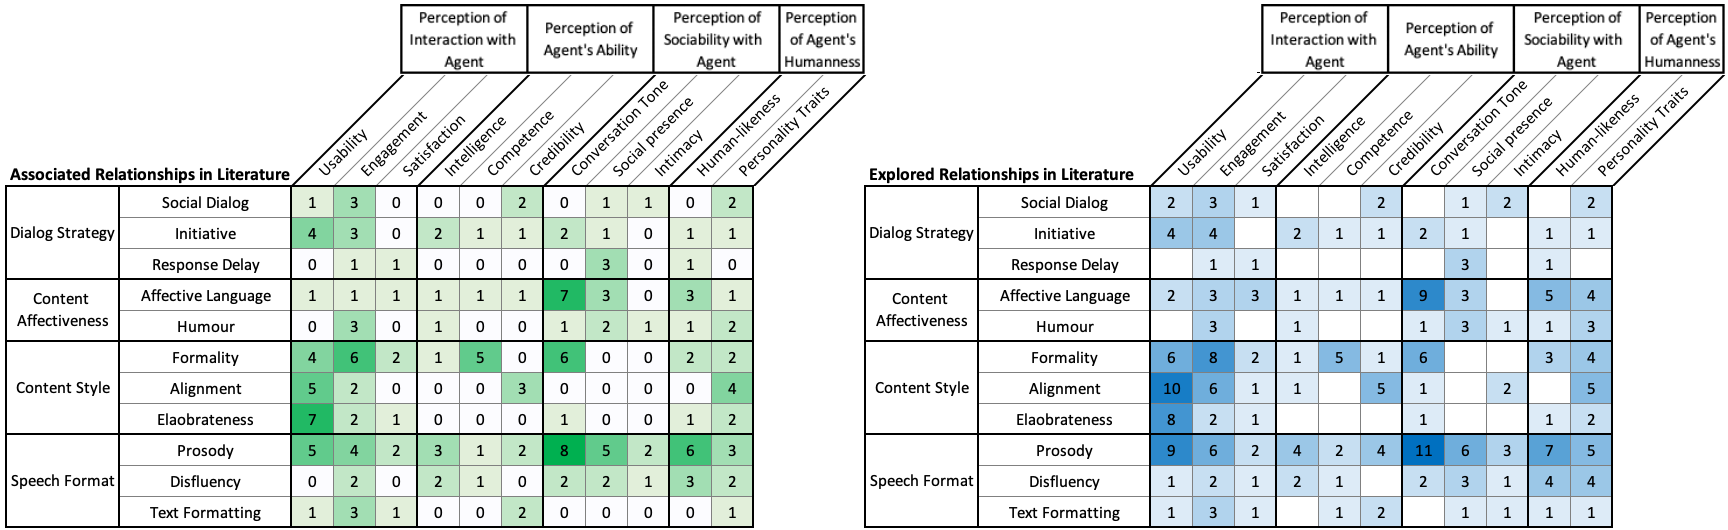
\includegraphics[width=\textwidth]{fig-heatmap-coverage.png}
  \caption{Heatmap of literature for perception of conversational agents for each type of conversational architecture element}
  \label{fig:heatmap-coverage}
\end{figure*}

\subsubsection{Perception of Agent's Ability}

The effects of conversation architecture elements on the perception of agent's ability is the least explored connection in the corpus (n=35). Out of these explored connections, 27 relationships had an effect between the studied architecture elements and ability perceptions. For these impactful relationships, the corpus had similar numbers of connections across voice-based (n=15) and text-based (n=12) CAs.

Across the themes in this perception category, \textbf{competence} had the smallest number of relationships in our corpus compared to intelligence and trust. Some studies discussed that the perception of competence is dependent various influencing factors, such as task difficulty \cite{kraus2020effects}\cmt{[64]}. Overall, studies on the perception of \textbf{intelligence} had impactful results, such as the use of formal language made the CA seem more knowledgeable \cite{volkel2022user}\cmt{[75]}. However, some evidence suggest that there are nuances to this perception, as a filler-speaking agent was perceived as less intelligent in task-oriented conditions, but was seen as slightly more intelligent in social-oriented conditions \cite{jeong2019exploring}\cmt{[10]}.

For the conversation architecture categories related to the perception of agent's ability, all 10 explored connections related to \textbf{linguistic content} had impacted user's perception. Specifically, CAs utilizing \textbf{agent-initiative content} such as using proactive dialogue and conversation repair strategies are seen as more competent \cite{kraus2020effects}\cmt{[64]} and intelligent \cite{ashktorab2019resilient}\cmt{[88]}. However, the effect of being proactive on user's trust with an agent may be dependent on the proactive style of the user's own conversation patterns \cite{kraus2020effects}\cmt{[64]}. For CAs using \textbf{affective language}, some studies found that using more expressive words increased intelligence and competence \cite{lee2019s}\cmt{[55]}\cite{yang2017perceived}\cmt{[44]}, but it may decrease the perceived trustworthiness of an agent 
%as discussed in Healey et al's study using an agent with an encouraging personality
\cite{healey2013relating}\cmt{[39]}.

The conversation architecture categories \textbf{Linguistic style} and \textbf{non-linguistic format} had mixed results, with some elements demonstrating relationships with the perception of the agent's abilities, while some others didn't. Most these mixed results came from relationships with the perception of trust. Studies with \textbf{alignment} found differences in trust rating in the interaction studies \cite{hoegen2019end}\cmt{[31]}, while some others did not reveal any differences \cite{huiyang2022improving}\cmt{[17]}. Also, research method may impact the perception of trust, as an observation study and interaction study on a similar topic yielded different results on the perception of trust \cite{linnemann2018can}\cmt{[15]}. The use of \textbf{prosodic cues} also had varied impacts on trust, as one study found that differences in vocal cues lead to a difference in perceived truthfulness \cite{dubiel2020persuasive}\cmt{[60]}, while another study using gendered voices did not find any statistically significant differences in perceived trust \cite{jestin2022effects}\cmt{[81]}.

\subsubsection{Perception of Social Connection with Agent}

There are 53 explored connections between conversation architecture elements and the perception of social connection with agents, with majority of them (n=40) resulted in relationships with effects. Interestingly, studies explored more perceptions of social connection with agent related to voice-based CAs (n=34) compared to text-based CAs (n=19), potentially due to the assumption that voice-based agents is more suitable to cultivate human-agent relationships. There are some mixed results for voice-based CAs, as 10 out of the 34 connections did not find any significant results. Half of the neutral results come from the conversation architecture element of \textbf{prosodic cues}. For example, the pitch of agents' voices did not impact the perceived rapport \cite{lubold2016effects}\cmt{[86]} between agent and users or the appropriateness of tone \cite{jestin2022effects}\cmt{[81]}. However, there are also findings that the use of vocal cues made the agent sound more empathetic \cite{tolmeijer2021female}\cmt{[62]}, as well as increased perceived emotional connection \cite{chan2021kinvoices}\cmt{[74]}\cite{kim2020can}\cmt{[24]}. This shows that there are nuanced factors within prosodic cues that impact the perception of social connections that we have not captured in our relationships.

Across the themes in this perception category, \textbf{social presence} (n=17) and \textbf{conversation tone} (n=18) have similar number of relationships between architecture elements and perceptions, but \textbf{intimacy} (n=5) has less number of impactful relationships. One reason for this is half of the explored connections did not have any effect on the perception of social connection, such as the use of capitalization \cite{westerman2019believe}\cmt{[9]}, lexical alignment \cite{linnemann2018can}\cmt{[15]}, or social dialogue \cite{lubold2016effects}\cmt{[86]}. For \textbf{social presence}, conversation architecture elements from \textbf{non-linguistic format} category, prosodic cue and text variation, had a number of impactful relationships in the reviewed studies. For example, participants conversing with the agents using kin's voices experienced significantly higher perceived co-presence where there is a closer psychological connection with the agent \cite{chan2021kinvoices}\cmt{[74]}. Also, text-based agents including a delay before responding to users were rated higher in social presence ratings compared to the agent that did not use any response delays \cite{gnewuch2018faster}\cmt{[19]}\cite{gnewuch2022opposing}\cmt{[20]}. Lastly, the use of \textbf{prosodic cues} can impact the perceived \textbf{conversation tone} of the agent as emotionally expressive \cite{zhu2022effects}\cmt{[26]} or persuasive \cite{chan2021kinvoices}\cmt{[74]}, as well as the appropriateness of the tone used by the agent \cite{jestin2022effects}\cmt{[81]}\cite{misu2011toward}\cmt{[83]}.

Looking at the different categories of conversation architecture cues, the heatmap (Figure \ref{fig:heatmap-impact} shows that there are not many relationships in \textbf{linguistic style} that are related to the perceived social connection with CAs. There are not many explored connections in our reviewed corpus between the two, which could be an indication of the assumption that linguistic style does not impact the perception of social connections.
While we discussed the impact of non-linguistic elements of prosodic cues and text variations earlier, the conversation architecture elements in the linguistic content category also had effects on the perception of social connections. Specifically, CAs using of \textbf{affective language} were perceived to be more empathetic \cite{daher2020empathic}\cmt{[58]}\cite{diederich2019emulating}\cmt{[25]}\cite{yang2017perceived}\cmt{[44]} and emotionally expressive \cite{zhu2022effects}\cmt{[26]}, and emotional connection with the agent \cite{lee2019s}\cmt{[55]}\cite{lubis2019positive}\cmt{[43]}.

%add text variation in the discussion

\subsubsection{Perception of Agent's Humanness}

Agent's humanness is the second most explored perception within our reviewed corpus (n=76), with majority of the connections finding impacted relationship between the studied conversation architecture elements and the perception of agent's humanness (n=56). While the connections were explored more for voice-based agent (n=49) as compared to text-based agents (n=27), the actual impacted relationships between the modalities were similar (voice=32, text=24). This is due to larger number of neutral relationships within voice modality, such as the use of affective language for a speech agent did not impact its perceived likeability \cite{hu2022polite}\cmt{[76]}.

Across the themes in this perception category, both \textbf{human-likeness} and \textbf{personality traits} have relationships with almost all conversation architecture elements. Based on the reviewed corpus, it seems like all the conversation architecture elements extracted from literature have some impact on the perception of agent's humanness. However, the impacts can be both positive or negative. In the case of Chan et al's study \cite{chan2021kinvoices}\cmt{[74]}, participated rated the agent using kin voices as significantly more likeable compared to the generic voices, but it was perceived as eerie. As for the perceptions within this category, there are more relationships for perceived personality traits (n=33) vs. human-likeness (n=18). This is because many studies only have one measure for human-likeness (e.g. artificial or human-like), but have multiple aspects of personality to be explored. For example, participant rated the agent using affective language as more polite, as well as reflected that the agent seemed friendly \cite{hu2022polite}\cmt{[76]}. 

For the conversation architecture elements, formality in the linguistic style category and prosodic cue in the non-linguistic format category had more effects on the perception of agent's humanness in the reviewed corpus. For \textbf{formality}, agents using casual style is perceived as more human-like with a warm, kind and entertaining personality \cite{cox2022does}\cmt{[27]}\cite{jestin2022effects}\cmt{[81]}\cite{kim2019comparing}\cmt{[89]}. The use of \textbf{prosodic cues} varying pitch, intonation and speech rate of a conversation agent generally had impacts on the perceived humanness instead of personality traits \cite{choi2020nobody}\cmt{[54]}\cite{jestin2022effects}\cmt{[81]}\cite{misu2011toward}\cmt{[83]}. For the architecture elements of \textbf{disfluency}, the type of impact on the perception of humanness depended on the context of the conversation. Studies have found that participants perceived the filler-condition agent as more likeable in the social-oriented situation, but did not find the same effect in task-oriented situations \cite{jeong2019exploring}\cmt{[10]}\cite{wester2015artificial}\cmt{[14]}.





%-------------
\section{Discussions}

\subsection{Research Challenges and Opportunities}

%Three major needs emerged from the trends identified by our review: 1) 2) 3).

\subsubsection{Inconsistencies in Perception Measures}

A major roadblock in synthesizing the findings from existing academic research is the diversity and inconsistency of measurements towards the anthropomorphized perception of agents. It is difficult to assess whether perception measures should be compared with each other. Also, some measures combined anthropomorphized perceptions into a composite score, which makes it impossible to separate the perceptions into more granular details.

Based on the literature reviewed in this paper, we noticed that similar perception concepts were \textbf{measured in different ways} through different surveys. For example, there are several approaches to measure the perceived \textit{human-likeness} of an agent. A commonly used survey is adapted from the Godspeed questionnaire \cite{bartneck2009measurement}, which measures human-likeness based on user's impression of the agent as fake / natural, machinelike / humanlike, unconscious / conscious, and artificial / lifelike (used by \cite{hoegen2019end}\cmt{[31]}, \cite{jeong2019exploring}\cmt{[10]} and \cite{ouchi2019should}\cmt{[59]}). Another way to measure human-likeness is adapted from Holtgraves et al.'s \cite{holtgraves2007perceiving} questionnaire, which asks users to assess the agent's perceived human-likeness, skillfulness, thoughtfulness, politeness, responsiveness and engagement (used by \cite{diederich2019emulating}\cmt{[25]} and  \cite{gnewuch2018faster}\cmt{[19]}). One study \cite{westerman2019believe}\cmt{[9]} used the Ascend of Man pictorial scale \cite{kteily2015ascent} as the measure of perceived human-likeness. It is unclear whether these different measures of perceived human-likeness are similar enough to be compared with each other.

 In addition to different methods used to measure for the same perception, our detailed analysis revealed that the measures using the same label may have \textbf{different meanings}. In Diedrech et al.'s study \cite{diederich2019emulating}\cmt{[25]}, \textit{empathy} measure is adapted from \cite{yan2013role} assessing whether the CA gives users individual or personal attention. In Daher et al.'s study \cite{daher2020empathic}\cmt{[58]}, they also measure the perception of empathy, but it is using the RoPE Scale \cite{charrier2019rope} with questions like "the robot cares about my feelings" or "the robot comforts me when I am upset." These two different measures of empathy seem to have different underlying meanings, one assessing the personalization aspect of CAs, while the other is assessing the emotional aspect of CAs. Another example is the measurement of \textit{trustworthiness}, with some constructs measuring the level of sensitive information user's are willing to share \cite{dinev2006privacy}, and some measuring the honesty and truthfulness of an agent \cite{lee2017enhancing}. 

Lastly, there are \textbf{composite measures} of anthropomorphized perception across different categories, making it difficult to break down perceptions into granular details for analysis. One such example is Ma et al's study \cite{ma2022ask}\cmt{[29]} on different approaches for CAs to reply to users' uncertain queries. UX score is used to measure the perception of an agent, which asks whether the user thinks the CA's response is pleasing / trustworthy / natural / acceptable / shorten the distance between CA and user. While the study has found significant impact of the use of formal language on UX score, it is not possible to breakdown the measure into perceptions of interaction (pleasing, acceptable), social connection (shorten the distance between CA and user), and humanness (natural, trustworthy). Similar for Hoegen et al.'s study \cite{hoegen2019end}\cmt{[31]} on the impact of conversational style matching, it is not possible to separate the overall interaction score into different perceptions as the composite measure contains questions measuring different categories of perceptions like interaction (engaging) and humanness (trust, likable).

In recent years there has been some effort towards unifying the evaluation of conversational agents, such as the work by Finch et al. \cite{finch2020towards} presenting a comprehensive analysis of current evaluation protocols. More work is needed to categorize and consolidate perception measures to make them consistent and comparable across various studies. 


\subsubsection{Nuances in Influencing Factors}

While the discussion in the Framework section above focuses on the overall effect of conversational architecture elements on anthropomorphized perceptions,  there are other nuanced influencing factors that impact user perceptions of agents. 

Depending on the \textbf{type of conversation} user is having with agents, it may lead to differences in perceptions for similar conversational architecture elements. Cox et al. \cite{cox2022does}\cmt{[27]} found that the perceived competence and appropriateness of tone of different language formality styles depend on the sensitivity of information discussed in the conversation. In this particular study, a formal language style is preferred in medical history discussions as it is matching to the expectation of users, but there is no difference in perception between formal and casual styles when discussing income level and credit scores. In Jeong et al's study \cite{jeong2019exploring}\cmt{[10]}, users found the agent using fillers less intelligent and likable in a task-oriented conversation, but found the same agent using fillers as slight more intelligent and likable in a social-oriented conversation. Another factor that could impact perceptions is the \textbf{anonymity} of conversation. Based on user feedback, Lee et al. \cite{lee2020hear}\cmt{[23]} found that the anonymity of a conversational agent is a driving factor encouraging people to self disclose without having to worried about judgements from the CA. The perception of the agent may be different if the user's identity is not anonymous.

Other than the type of conversation, \textbf{user's characteristics} can also be influencing factors on their perception of agents. For example, the effect of matching user's conversational style on perception of agents depend on user's own conversational style, as participants with high consideration conversational style rated the lexically aligned agent as more trustworthy \cite{hoegen2019end}\cmt{[31]}. In the study by Cox et al. \cite{cox2022does}\cmt{[27]}, participants with lower levels of privacy concerns as well as those who believe in robotic intelligence found the chatbot more enjoyable, warm, competent and appropriate. Similarly, participants with positive attitudes towards computers were significantly more likely to indicate that the usage of fillers by agents was a positive aspect of the conversation, compared to participants with neutral attitudes towards computers \cite{pfeifer2009should}\cmt{[12]}. Lastly, user's prior experience with conversational agents could impact perception of agents. Experienced users perceived the agent with a response delay as lower in social presence compared to the one without delay, as it is seen as inefficient to wait for the CA to respond. However, novice users perceived higher social presence conversing with the CAs using response delays as it is more similar to conversations with human partners \cite{gnewuch2018faster}\cmt{[19]}.


%Designing for personalities, not individual elements

%* The size of the effect for language we observed is clearly higher than the size of the effect for voice. \cite{habler2019effects}\cmt{[63]}

%Combined effects
%* integrated mental model \cite{knijnenburg2016inferring}\cmt{[34]}
%* Anthropomorphized chatbot (text) using affective language (emotional expressions), self-referencing, emoticons, response delays. Resulted in higher perceived anthropomorphism, which in result led to lower negative word of mouth and loss of trust. anthropomorphic design is beneficial not only to initial trust but also to the ongoing trust relationship \cite{seeger2021chatbots}\cmt{[35]}

%For discussions on mental well beings, agent using emojis is rated higher for attitude (emotional connection) . However, for agent with discussing physical well being, agent using emojis is rated as lower for attitude. 
%Attitude has emotional connection, coherent - coherent is an ability perception, vs. emotional connection is a social connection perception. \cite{fadhil2018effect}\cmt{[52]}

%* Format: Response delay - Novice users perceived the agent as more socially present, but experienced users had a negative effect \cite{gnewuch2022opposing}\cmt{[20]}
%* Content: Humour - no overall significant difference between conventional method vs. agent using humour for enjoyment. Specifically, men enjoyed the agent's jokes more than women.  \cite{miyamoto2017improving}\cmt{[46]}.
%* Format: Proactivity - significant interaction between proactive dialogue strategies and task difficulty for perceived competence and perceived reliability. For easier tasks, system help is not really required. \cite{kraus2020effects}\cmt{[64]}
%* Preference for the level of social talk depended on the task, even within the same transactional context, as users preferred high level for playing a song, but low level for writing a text. \cite{volkel2021manipulating}\cmt{[68]}
%* Correlation between user's personality of agreeableness vs. preference for agreeable level of chatbot \cite{volkel2021examining}\cmt{[69]}
%* For expertise, multilingual students rated higher the non-native English-speaking virtual human. \cite{feijoo2021effects}\cmt{[70]}
%* Participants felt irritated when humorous statements were made when they talked about experiencing sadness \cite{go2021conversational}\cmt{[80]}

%\subsubsection{Study Design}

%\textbf{Interview vs experiment}
%* Humour - what's said vs. study results

%\textbf{Observer study vs. interaction study}
%* In observer study, participants attributed higher integrity (trustworthiness), response accuracy and likeability to the agent with lexical alignment, but this effect was not observed in the interaction study. Also, interaction study had lower cognitive demand but no effect in the observer study. \cite{linnemann2018can}\cmt{[15]}
%* \cite{zhu2022effects}\cmt{[26]}
%* \cite{cox2022does}\cmt{[27]}

%* that a sense of intimate connection to the CA is more important than efficient task handling in some contexts \54
%* VA self-repair can backfire if time or accuracy is of the essence. (repair and accuracy) \cite{cuadra2021my}\cmt{[67]}

%Sometimes a study is covering multiple conversational element cues, hard to break it out. For example, extroverted personality used in \cite{volkel2022user}\cmt{[75]} has emoticons, affective language, talkative, and self-disclosure. Need to break it down.

%Also, breaking down "personalities" to its core components.

%There are a few studies that designed conversational agents composed with multiple conversation architecture elements. This is especially evident in studies comparing different personalities of CAs, such as extroverted vs. introverted. In Volkel et al's study, the personality of extraversion is a combination of linguistic content like social ta

%\cite{moilanen2022measuring}\cmt{[82]}\cite{seeger2021chatbots}\cmt{[35]}\cite{volkel2021manipulating}\cmt{[68]}\cite{volkel2022user}\cmt{[75]}.

\subsubsection{Consider Relationships Within Perceptions}

There are empirical evidence that different perceptions of agent have effects on each other. Moussawi et al \cite{moussawi2021perceptions}\cmt{[36]} conducted a study to understand the correlations between different perceptions impacting user's intention to adopt a conversational agent. Specifically, they found a correlation within the category of perceived ability, where perceived intelligence is positively correlated to initial trust of the agent. Also, the study found that users with higher perceived intelligence of an agent are more likely to attribute higher ratings for the perception category of interaction on the perceived ease of use and enjoyment, as well as higher ratings for perceived anthropomorphism. Perceived anthropomorphism have a positive impact on perceived enjoyment, which lead to higher intention to adopt the CA. This study outlines that the perception themes we identified in this paper are not independent of each other.

The correlations between perception measures are covered in a few of the papers in our corpus. In the study of using response delays, the perception of social presence had a significant effect on the intention to use \cite{gnewuch2022opposing}\cmt{[20]}. In another study, the CA's perceived personality trait of agreeableness has an influence on the perception of trust \cite{andrews2012system}\cmt{[38]}. Seeger et al's study had similar findings, where higher perceived anthropomorphism lead to lower loss of trust \cite{seeger2021chatbots}\cmt{[35]}. There are also effects within the same perception category, such as a speech agent that is rated higher in perceived human-likeness was associated with higher likability ratings \cite{zhu2022effects}\cmt{[26]}. Also, within the perception category of social connection, one study found that social distance is positively related to the perceived social attraction \cite{westerman2019believe}\cmt{[9]}. 

These correlations between perceptions demonstrate that designing for specific anthropomorphized perceptions of conversational agents is more nuanced than the sum of the impacts from individual perceptions. Perceptions have influences on each other, either within the same category or across different categories. However, there is not enough studied connections in existing literature to make a meaningful systematic analysis of the relationship within perceptions. More research is needed in this area to study these relationships, to understand whether there are systematic trends in the influences of perceptions, and whether there is a sequence of perceptions to achieve the desired overall anthropomorphized perception of agents.

\subsection{Ethical Considerations}

While the use of conversation architecture elements can be used to design anthropomorphized perceptions, it is important to address the potential ethical implications that could negative impact users. There are three items discussed in this section: societal stereotypes, influencing user's actions and privacy concerns.

For prosodic cues, there are various studies in our corpus exploring the effect of different pitches on different perceptions of agents. Even in studies not explicitly studying the effect of gendered voices in an agent, possible stereotypes may still exist in the study. Studies exploring the impact of gendered voices found that lower pitches usually associated with men are considered to be more desirable, authoritative but less friendly \cite{tolmeijer2021female}\cmt{[62]}\cite{jestin2022effects}\cmt{[81]}. For Dubiel et al's study \cite{dubiel2020persuasive}\cmt{[60]}, the prosody setting with the lower mean pitch was selected as the more persuasive voice through a user study. These results may be due to the unconscious bias to select a male sounding voice as more persuasive over female sounding voices that are usually using higher pitches. While some guidelines recommend designing agents to be androgynous to avoid gender stereotypes \cite{ruane2019conversational}, there are limitations in creating gender-ambiguous voices. Currently there is no defined aspects on what is perceived as a gender-neutral voice  \cite{jestin2022effects}\cmt{[81]}, and there is a lack of voice generators available to generate voices that are seen as androgynous \cite{tolmeijer2021female}\cmt{[62]}.

Conversation architecture elements can be used to design perceptions of agents to make the CA more persuasive. This opens up the ethical issue of influencing user's attitudes and behaviours through these persuasion techniques. In a study by Chan et al \cite{chan2021kinvoices}\cmt{[74]}, they found that CAs using kin's voices are perceived as more credible and likeable, with a higher perceived social presence with the agent. These perceptions contributes to the agent being more engaging and persuasive, therefore people are more likely to comply with its requests. Andrew et al \cite{andrews2012system}\cmt{[38]} found that tailoring the personality of the CA to users will positively impact an agent's persuasiveness. These persuasion techniques can be beneficial to help users achieve their goals, but can also be used for harmful actions, such as when trying to get someone to believe false information for their own gain.

Another key area of concern is privacy. Given the natural language format of conversational agents, users may be disclosing more sensitive and personal information than needed for the interaction. In relationship to conversation architecture, some elements like self-disclosure and using persuasive voices resulting in higher trust, leading participants to disclose sensitive information with the agent \cite{lee2020hear}\cmt{[23]}\cite{dubiel2020persuasive}\cmt{[60]}. This can expose users to attacks, such as CAs using voice impersonation to ask for personal information for malicious intents \cite{chan2021kinvoices}\cmt{[74]}. Designing for anthropomorphized perceptions of agents requires careful consideration of privacy issues including the sensitivity of the data, who has access to it, and how to protect against nefarious users.

\subsection{Limitations and Future Work}

Our systematic literature review was limited to papers published in the ACM Digital Library between 2010 and 2022. We may have missed literature published outside this time period, as well as in other libraries. Also, most of the studies in our corpus are based on lab experiments with short interactions. The generalizability of these findings need to be verified through longer term engagements with conversational agents deployed in real world situations. Lastly, research without empirical studies on the perception of agents are excluded based on our selection criteria. We may have missed some influential findings in these papers. To better understand the relationships between conversation architecture elements and anthropomorphized perceptions, we plan to conduct future reviews in literature and user studies to understand their real-world impacts.

\section{Conclusions}

In this paper, we discussed the results of a systematic review of existing literature published in the ACM Digital Library on the impact of conversation architecture elements on anthropomorphized perceptions of CAs.  Through our synthesis of our corpus of 57 papers, we have created a consistent taxonomy for perceptions of agents, as well as conversation architecture elements. Also, we have mapped the relationships between perceptions and conversation architecture to a generalized framework based on the impacts discussed in our reviewed corpus. Through our analysis, we have found that perception measures are being used inconsistently across studies, as well as other influencing factors on the perception of agents. We recommend future research to consider creating consistent measures that can explore different aspects of perceptions, as well as more explorations into the patterns behind other influencing factors that have impacts on anthropomorphized perceptions. While our research contribute to design conversation architecture to orchestrate specific anthropomorphized perceptions, we urge everyone to incorporate ethical perspectives into their design considerations.

%%
%% The acknowledgments section is defined using the "acks" environment
%% (and NOT an unnumbered section). This ensures the proper
%% identification of the section in the article metadata, and the
%% consistent spelling of the heading.
\begin{acks}
TBD
\end{acks}






%%
%% The next two lines define the bibliography style to be used, and
%% the bibliography file.
\bibliographystyle{ACM-Reference-Format}
\bibliography{references}

%%
%% If your work has an appendix, this is the place to put it.
\appendix

\end{document}
\endinput
%%
%% End of file `paper.tex'.